\documentclass{article}
\usepackage[preprint]{neurips_2024}
\usepackage[utf8]{inputenc}
\usepackage[T1]{fontenc}
\usepackage[colorlinks=true,linkcolor=black,citecolor=blue!50!black,urlcolor=blue!50!black]{hyperref}
\usepackage{url}
\usepackage{booktabs}
\usepackage{amsmath,amssymb,amsthm}
\usepackage{cancel}
\usepackage{microtype}
\usepackage{xcolor}
\usepackage{tikz}
\usetikzlibrary{arrows.meta,positioning}

\newtheorem{proposition}{Proposition}[section]
\newtheorem{lemma}[proposition]{Lemma}
\newtheorem{corollary}[proposition]{Corollary}
\theoremstyle{definition}
\newtheorem{definition}[proposition]{Definition}
\newtheorem{assumption}{Assumption}
\theoremstyle{remark}
\newtheorem{remark}[proposition]{Remark}
\newtheorem{example}[proposition]{Example}

\newcommand{\E}{\mathbb{E}}
\newcommand{\dE}{\Delta E}
\newcommand{\dP}{\Delta P}
\newcommand{\Ob}{\bar O}
\newcommand{\KL}{\mathrm{KL}}
\newcommand{\why}[1]{\tag*{\small(#1)}}

\title{The State Defect, Empowerment and Plasticity}

\author{XXX}

\begin{document}
\maketitle

\begin{abstract}
For an agent that acts on a memory, we derive the empowerment and plasticity mismatches between the history and the memory, the two splits of the state defect, and three ways to separate the reward inside them. We then relate the known condition under which a memory gives the value of every later policy, that it predicts the reward and its own next state as well as the history does, to the two splits, and, for a memory with few values, choose what it keeps by one objective after \citet{still2012information}. Every derivation is written term by term, and every cancellation names the assumption or lemma that allows it.
\end{abstract}

\section{Setting}\label{sec:setting}

\begin{center}
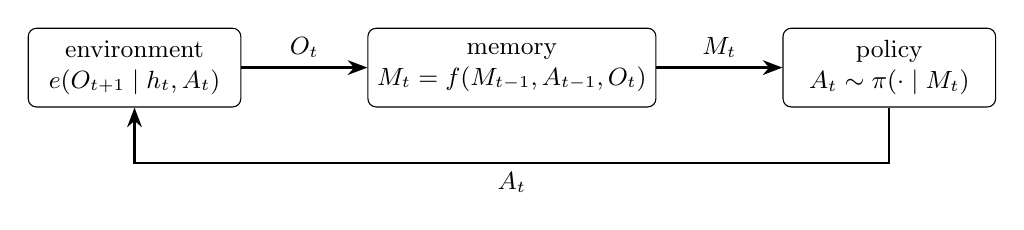
\begin{tikzpicture}[>={Stealth[length=2.5mm]}, node distance=10mm and 16mm,
  box/.style={draw, rounded corners=3pt, minimum height=10mm, minimum width=27mm, align=center, font=\small}]
\node[box] (world) {environment\\ $e(O_{t+1}\mid h_t, A_t)$};
\node[box, right=of world] (mem) {memory\\ $M_t = f(M_{t-1}, A_{t-1}, O_t)$};
\node[box, right=of mem] (pol) {policy\\ $A_t \sim \pi(\cdot \mid M_t)$};
\draw[->, thick] (world) -- node[above, font=\small] {$O_t$} (mem);
\draw[->, thick] (mem) -- node[above, font=\small] {$M_t$} (pol);
\draw[->, thick] (pol.south) -- ++(0,-7mm) -| node[pos=0.25, below, font=\small] {$A_t$} (world.south);
\end{tikzpicture}
\end{center}

The history is $h_t=(O_1,A_1,\dots,A_{t-1},O_t)$. The observation contains the reward: $O_t=(R_t,\Ob_t)$, with $\Ob_t$ the rest of the observation. All observation and action sets are finite, and all probabilities are under the law of the agent's experience induced by the three boxes.

\begin{assumption}[Environment]\label{as:env}
$O_{t+1}\sim e(\cdot\mid h_t,A_t)$ for some law $e$; the environment may depend on the whole history, with no Markov or stationarity condition.
\end{assumption}

\begin{assumption}[Memory]\label{as:mem}
$M_1=f_1(O_1)$ and $M_{t+1}=f(M_t,A_t,O_{t+1})$ for fixed maps $f_1,f$. Hence $M_t$ is a function of $h_t$.
\end{assumption}

\begin{assumption}[Policy]\label{as:pol}
$P(A_t=a\mid h_t)=\pi(a\mid M_t)$: the action depends on the history only through the memory.
\end{assumption}

Every numbered statement was checked numerically. The script \texttt{checks/verify\_note.py} computes the exact law of all trajectories in small random environments whose next observation depends on the whole history, in an environment built so that the conditions of Proposition~\ref{prop:every} hold, and in the examples; it tests each numbered statement for a finite horizon, and the largest error is $10^{-13}$.

\section{Tools}\label{sec:tools}

We use six standard facts \citep[Ch.~2]{cover2006elements}. $X,Y,W,Z$ are random variables, and conditioning on nothing is allowed.
\begin{enumerate}
\item[(T1)] $I(X;Y\mid Z)=H(X\mid Z)-H(X\mid Y,Z)=H(Y\mid Z)-H(Y\mid X,Z)$.
\item[(T2)] Chain rule: $I(X,Y;W\mid Z)=I(X;W\mid Z)+I(Y;W\mid Z,X)=I(Y;W\mid Z)+I(X;W\mid Z,Y)$, and the same with the pair in the second place, since $I$ is symmetric.
\item[(T3)] $I(X;Y\mid Z)\ge0$, with equality exactly when $X$ and $Y$ are independent given $Z$.
\item[(T4)] If $W$ is a function of $X$, conditioning on $(X,W)$ is the same as conditioning on $X$: $H(Y\mid X,W,Z)=H(Y\mid X,Z)$. By Assumption~\ref{as:mem}, this applies to $W=M_t$, $X=h_t$.
\item[(T5)] $h_{t+1}=(h_t,A_t,O_{t+1})$, so conditioning on $h_{t+1}$ is the same as conditioning on $(h_t,A_t,O_{t+1})$.
\item[(T6)] If $W$ is a function of $Z$, then $H(W\mid Z)=0$, and $I(X;W\mid Z)=0$ for every $X$, since by (T1) and (T3) $0\le I(X;W\mid Z)=H(W\mid Z)-H(W\mid X,Z)\le H(W\mid Z)$. By Assumption~\ref{as:mem}, this applies to $W=M_{t+1}$, $Z=(M_t,A_t,O_{t+1})$.
\end{enumerate}

\begin{lemma}[The action depends on the past only through the memory]\label{lem:action}
Under Assumptions~\ref{as:mem} and~\ref{as:pol}, for every $k\ge0$,
\[
H(A_{t+k}\mid h_t,A_t,O_{t+1},\dots,A_{t+k-1},O_{t+k})=H(A_{t+k}\mid M_t,A_t,O_{t+1},\dots,A_{t+k-1},O_{t+k}),
\]
and therefore $I(h_t;A_{t+k}\mid M_t,A_t,O_{t+1},\dots,A_{t+k-1},O_{t+k})=0$. The cases used most are
\begin{align*}
\text{(a) } k=0:&\quad H(A_t\mid h_t)=H(A_t\mid M_t),\\
\text{(b) } k=1:&\quad H(A_{t+1}\mid h_t,A_t,O_{t+1})=H(A_{t+1}\mid M_t,A_t,O_{t+1}).
\end{align*}
\end{lemma}

\begin{proof}
By (T5) applied $k$ times, the conditioning variables on the left are $h_{t+k}$. By Assumption~\ref{as:pol}, the law of $A_{t+k}$ given $h_{t+k}$ is $\pi(\cdot\mid M_{t+k})$. By Assumption~\ref{as:mem}, $M_{t+k}$ is obtained from $M_t$ by applying $f$ $k$ times with the inputs $(A_t,O_{t+1}),\dots,(A_{t+k-1},O_{t+k})$, so it is a function of the conditioning variables on the right. These variables are a function of $h_{t+k}$, so the law of $A_{t+k}$ given them is the average of $\pi(\cdot\mid M_{t+k})$ over the histories consistent with them, which is $\pi(\cdot\mid M_{t+k})$ itself. Both laws are $\pi(\cdot\mid M_{t+k})$, so the two entropies are equal. For the mutual information, write $C=(A_t,O_{t+1},\dots,A_{t+k-1},O_{t+k})$ in this proof only:
\begin{align*}
I(h_t;A_{t+k}\mid M_t,C)
&=H(A_{t+k}\mid M_t,C)-H(A_{t+k}\mid h_t,M_t,C) \why{T1}\\
&=H(A_{t+k}\mid M_t,C)-H(A_{t+k}\mid h_t,C) \why{T4}\\
&=0 \why{the equality of entropies above}.
\end{align*}
\end{proof}
\section{Empowerment and plasticity at the history and at the memory}\label{sec:EP}

In every derivation below, the label at the right of a line names the fact used to obtain that line. Two struck-through terms in a line are equal by the named fact and cancel.

\begin{definition}\label{def:EP}
Following the one-step form of \citet{abel2025plasticity}, the empowerment of the action and the plasticity of the next action, computed from the history and from the memory, are
\begin{align*}
E_t&=I(A_t;O_{t+1}\mid h_t), & E_t(M)&=I(A_t;O_{t+1}\mid M_t),\\
P_{t+1}&=I(O_{t+1};A_{t+1}\mid h_t,A_t), & P_{t+1}(M)&=I(O_{t+1};A_{t+1}\mid M_t,A_t),
\end{align*}
and the two mismatches are $\dE_t=E_t-E_t(M)$ and $\dP_t=P_{t+1}(M)-P_{t+1}$.
\end{definition}

\begin{proposition}[Empowerment mismatch]\label{prop:dE}
Under Assumptions~\ref{as:mem} and~\ref{as:pol}, $\dE_t=I(h_t;A_t\mid M_t,O_{t+1})\ge0$.
\end{proposition}

\begin{proof}
Write both empowerments with (T1), with $A_t$ as the variable whose entropy is taken:
\begin{align*}
E_t&=H(A_t\mid h_t)-H(A_t\mid h_t,O_{t+1}),\\
E_t(M)&=H(A_t\mid M_t)-H(A_t\mid M_t,O_{t+1}).
\end{align*}
Subtract:
\begin{align*}
\dE_t&=\cancel{H(A_t\mid h_t)}-H(A_t\mid h_t,O_{t+1})-\cancel{H(A_t\mid M_t)}+H(A_t\mid M_t,O_{t+1}) \why{struck terms equal, Lemma~\ref{lem:action}(a)}\\
&=H(A_t\mid M_t,O_{t+1})-H(A_t\mid h_t,O_{t+1})\\
&=H(A_t\mid M_t,O_{t+1})-H(A_t\mid h_t,M_t,O_{t+1}) \why{T4}\\
&=I(h_t;A_t\mid M_t,O_{t+1}) \why{T1},
\end{align*}
which is nonnegative by (T3).
\end{proof}

\begin{proposition}[Plasticity mismatch]\label{prop:dP}
Under Assumptions~\ref{as:mem} and~\ref{as:pol}, $\dP_t=I(h_t;A_{t+1}\mid M_t,A_t)\ge0$.
\end{proposition}

\begin{proof}
Write both plasticities with (T1), with $A_{t+1}$ as the variable whose entropy is taken:
\begin{align*}
P_{t+1}&=H(A_{t+1}\mid h_t,A_t)-H(A_{t+1}\mid h_t,A_t,O_{t+1}),\\
P_{t+1}(M)&=H(A_{t+1}\mid M_t,A_t)-H(A_{t+1}\mid M_t,A_t,O_{t+1}).
\end{align*}
Subtract:
\begin{align*}
\dP_t&=H(A_{t+1}\mid M_t,A_t)-\cancel{H(A_{t+1}\mid M_t,A_t,O_{t+1})}\\
&\quad-H(A_{t+1}\mid h_t,A_t)+\cancel{H(A_{t+1}\mid h_t,A_t,O_{t+1})} \why{struck terms equal, Lemma~\ref{lem:action}(b)}\\
&=H(A_{t+1}\mid M_t,A_t)-H(A_{t+1}\mid h_t,A_t)\\
&=H(A_{t+1}\mid M_t,A_t)-H(A_{t+1}\mid h_t,M_t,A_t) \why{T4}\\
&=I(h_t;A_{t+1}\mid M_t,A_t) \why{T1},
\end{align*}
which is nonnegative by (T3).
\end{proof}

In words: given the outcome, the history still tells something about the action that the memory does not, so the memory underestimates empowerment; and the history tells something about the next action that the memory does not, so the memory overestimates plasticity.

\section{The state defect and its two splits}\label{sec:splits}

\begin{definition}\label{def:terms}
The state defect and two further terms are
\[
D_t=I(h_t;O_{t+1}\mid M_t,A_t),\qquad D^0_t=I(h_t;O_{t+1}\mid M_t),\qquad D^+_t=I(h_t;O_{t+1}\mid M_t,A_t,A_{t+1}).
\]
With Propositions~\ref{prop:dE} and~\ref{prop:dP}, each of the five terms is a mutual information between the history and one variable, given the memory and other variables:
\begin{center}
\small
\begin{tabular}{llll}
\toprule
term & mutual information & variable predicted & given, besides $M_t$\\
\midrule
$D_t$ & $I(h_t;O_{t+1}\mid M_t,A_t)$ & $O_{t+1}$ & $A_t$\\
$D^0_t$ & $I(h_t;O_{t+1}\mid M_t)$ & $O_{t+1}$ & nothing\\
$\dE_t$ & $I(h_t;A_t\mid M_t,O_{t+1})$ & $A_t$ & $O_{t+1}$\\
$\dP_t$ & $I(h_t;A_{t+1}\mid M_t,A_t)$ & $A_{t+1}$ & $A_t$\\
$D^+_t$ & $I(h_t;O_{t+1}\mid M_t,A_t,A_{t+1})$ & $O_{t+1}$ & $A_t,A_{t+1}$\\
\bottomrule
\end{tabular}
\end{center}
By (T1) and (T4), each is the uncertainty about the predicted variable given the memory minus the uncertainty given the history.
\end{definition}

\begin{proposition}[First split]\label{prop:split1}
Under Assumptions~\ref{as:mem} and~\ref{as:pol}, $D_t=D^0_t+\dE_t$.
\end{proposition}

\begin{proof}
Apply (T2) to $I(h_t,A_t;O_{t+1}\mid M_t)$ in the two orders.

History first:
\begin{align*}
I(h_t,A_t;O_{t+1}\mid M_t)&=I(h_t;O_{t+1}\mid M_t)+I(A_t;O_{t+1}\mid M_t,h_t) \why{T2}\\
&=D^0_t+I(A_t;O_{t+1}\mid h_t) \why{Definition~\ref{def:terms}; T4}\\
&=D^0_t+E_t \why{Definition~\ref{def:EP}}.
\end{align*}
Action first:
\begin{align*}
I(h_t,A_t;O_{t+1}\mid M_t)&=I(A_t;O_{t+1}\mid M_t)+I(h_t;O_{t+1}\mid M_t,A_t) \why{T2}\\
&=E_t(M)+D_t \why{Definitions~\ref{def:EP} and~\ref{def:terms}}.
\end{align*}
The two right sides are equal, so $D^0_t+E_t=E_t(M)+D_t$, that is, $D_t=D^0_t+E_t-E_t(M)=D^0_t+\dE_t$.
\end{proof}

\begin{proposition}[Second split]\label{prop:split2}
Under Assumptions~\ref{as:mem} and~\ref{as:pol}, $D_t=\dP_t+D^+_t$.
\end{proposition}

\begin{proof}
Apply (T2) to $I(h_t;O_{t+1},A_{t+1}\mid M_t,A_t)$ in the two orders.

Next observation first:
\begin{align*}
I(h_t;O_{t+1},A_{t+1}\mid M_t,A_t)&=I(h_t;O_{t+1}\mid M_t,A_t)+I(h_t;A_{t+1}\mid M_t,A_t,O_{t+1}) \why{T2}\\
&=D_t+0 \why{Definition~\ref{def:terms}; Lemma~\ref{lem:action}, $k=1$}.
\end{align*}
Next action first:
\begin{align*}
I(h_t;O_{t+1},A_{t+1}\mid M_t,A_t)&=I(h_t;A_{t+1}\mid M_t,A_t)+I(h_t;O_{t+1}\mid M_t,A_t,A_{t+1}) \why{T2}\\
&=\dP_t+D^+_t \why{Proposition~\ref{prop:dP}; Definition~\ref{def:terms}}.
\end{align*}
The two right sides are equal.
\end{proof}

\begin{remark}[Both splits come from one quantity]\label{rem:orders}
Apply (T2) to $I(h_t;A_t,O_{t+1},A_{t+1}\mid M_t)$ in three orders. In the order of time, $(A_t,O_{t+1},A_{t+1})$, the terms are $I(h_t;A_t\mid M_t)=0$ (Lemma~\ref{lem:action}, $k=0$), $D_t$, and $I(h_t;A_{t+1}\mid M_t,A_t,O_{t+1})=0$ (Lemma~\ref{lem:action}, $k=1$). In the order $(O_{t+1},A_t,A_{t+1})$ they are $D^0_t$, $\dE_t$ and $I(h_t;A_{t+1}\mid M_t,O_{t+1},A_t)=0$. In the order $(A_t,A_{t+1},O_{t+1})$ they are $0$, $\dP_t$ and $D^+_t$. So the first split reads the action $A_t$ after the observation it produced, the second reads the next action $A_{t+1}$ before the observation it responds to, and in the order of time the two actions contribute nothing.
\end{remark}

\begin{corollary}\label{cor:consequences}
Under Assumptions~\ref{as:mem} and~\ref{as:pol}:
\begin{enumerate}
\item[(a)] $D_t=0$ if and only if $D^0_t=0$ and $\dE_t=0$, and if and only if $\dP_t=0$ and $D^+_t=0$;
\item[(b)] $\dP_t\le D_t$;
\item[(c)] $\dE_t\le H(A_t\mid M_t)$, so $\dE_t=0$ and $D_t=D^0_t$ when the policy is deterministic.
\end{enumerate}
\end{corollary}

\begin{proof}
(a) Each term is nonnegative (T3), and a sum of two nonnegative terms is zero exactly when both are. (b) From Proposition~\ref{prop:split2}, since $D^+_t\ge0$. (c) $\dE_t=H(A_t\mid M_t,O_{t+1})-H(A_t\mid h_t,O_{t+1})\le H(A_t\mid M_t,O_{t+1})\le H(A_t\mid M_t)$, where the first step drops a nonnegative entropy and the second uses that conditioning does not increase entropy, which is (T1) with (T3). A deterministic policy has $H(A_t\mid M_t)=0$; then Proposition~\ref{prop:split1} gives $D_t=D^0_t$.
\end{proof}

\section{Separating the reward}\label{sec:reward}

The observation is a pair, $O_{t+1}=(R_{t+1},\Ob_{t+1})$. We first split each term by a general pair $O_{t+1}=(X,Y)$, with $X$ taken first, and then consider three ways to separate the reward: reward first, $(X,Y)=(R_{t+1},\Ob_{t+1})$; rest first, $(X,Y)=(\Ob_{t+1},R_{t+1})$; and a partial information decomposition, which takes no order.

\subsection{A split by $O_{t+1}=(X,Y)$}

\begin{proposition}[$D_t$, $D^0_t$ and $D^+_t$]\label{prop:xy-D}
For $O_{t+1}=(X,Y)$,
\begin{align*}
D_t&=I(h_t;X\mid M_t,A_t)+I(h_t;Y\mid M_t,A_t,X),\\
D^0_t&=I(h_t;X\mid M_t)+I(h_t;Y\mid M_t,X),\\
D^+_t&=I(h_t;X\mid M_t,A_t,A_{t+1})+I(h_t;Y\mid M_t,A_t,A_{t+1},X),
\end{align*}
and every term on the right is nonnegative.
\end{proposition}

\begin{proof}
Each line is (T2) applied to $I(h_t;X,Y\mid\cdot)$ with $X$ first, and each term is nonnegative by (T3).
\end{proof}

\begin{proposition}[$\dE_t$]\label{prop:xy-E}
Under Assumptions~\ref{as:mem} and~\ref{as:pol}, for $O_{t+1}=(X,Y)$,
\[
\dE_t=\underbrace{\big[I(A_t;X\mid h_t)-I(A_t;X\mid M_t)\big]}_{X\text{ part}}+\underbrace{\big[I(A_t;Y\mid h_t,X)-I(A_t;Y\mid M_t,X)\big]}_{Y\text{ part}},
\]
where the $X$ part equals $I(h_t;A_t\mid M_t,X)\ge0$ and the $Y$ part can be negative.
\end{proposition}

\begin{proof}
By (T2), with $X$ first,
\begin{align*}
E_t&=I(A_t;X,Y\mid h_t)=I(A_t;X\mid h_t)+I(A_t;Y\mid h_t,X),\\
E_t(M)&=I(A_t;X,Y\mid M_t)=I(A_t;X\mid M_t)+I(A_t;Y\mid M_t,X).
\end{align*}
Subtracting and grouping the $X$ terms and the $Y$ terms gives the formula for $\dE_t=E_t-E_t(M)$. For the $X$ part, write both terms with (T1), with $A_t$ as the variable whose entropy is taken:
\begin{align*}
&I(A_t;X\mid h_t)-I(A_t;X\mid M_t)\\
&\quad=\cancel{H(A_t\mid h_t)}-H(A_t\mid h_t,X)-\cancel{H(A_t\mid M_t)}+H(A_t\mid M_t,X) \why{struck terms equal, Lemma~\ref{lem:action}(a)}\\
&\quad=H(A_t\mid M_t,X)-H(A_t\mid h_t,M_t,X) \why{T4}\\
&\quad=I(h_t;A_t\mid M_t,X) \why{T1}.
\end{align*}
The $Y$ part is a difference of two mutual informations with different conditioning, and no lemma relates them.
\end{proof}

\begin{proposition}[$\dP_t$]\label{prop:xy-P}
Under Assumptions~\ref{as:mem} and~\ref{as:pol}, for $O_{t+1}=(X,Y)$,
\[
\begin{aligned}
\dP_t&=\underbrace{\big[I(X;A_{t+1}\mid M_t,A_t)-I(X;A_{t+1}\mid h_t,A_t)\big]}_{X\text{ part}}\\
&\quad+\underbrace{\big[I(Y;A_{t+1}\mid M_t,A_t,X)-I(Y;A_{t+1}\mid h_t,A_t,X)\big]}_{Y\text{ part}},
\end{aligned}
\]
where the $Y$ part equals $I(h_t;A_{t+1}\mid M_t,A_t,X)\ge0$ and the $X$ part can be negative.
\end{proposition}

\begin{proof}
By (T2), with $X$ first,
\begin{align*}
P_{t+1}&=I(X,Y;A_{t+1}\mid h_t,A_t)=I(X;A_{t+1}\mid h_t,A_t)+I(Y;A_{t+1}\mid h_t,A_t,X),\\
P_{t+1}(M)&=I(X,Y;A_{t+1}\mid M_t,A_t)=I(X;A_{t+1}\mid M_t,A_t)+I(Y;A_{t+1}\mid M_t,A_t,X).
\end{align*}
Subtracting gives the formula for $\dP_t=P_{t+1}(M)-P_{t+1}$. For the $Y$ part, write both terms with (T1), with $A_{t+1}$ as the variable whose entropy is taken, and use $(X,Y)=O_{t+1}$:
\begin{align*}
&I(Y;A_{t+1}\mid M_t,A_t,X)-I(Y;A_{t+1}\mid h_t,A_t,X)\\
&\quad=H(A_{t+1}\mid M_t,A_t,X)-\cancel{H(A_{t+1}\mid M_t,A_t,O_{t+1})}\\
&\qquad-H(A_{t+1}\mid h_t,A_t,X)+\cancel{H(A_{t+1}\mid h_t,A_t,O_{t+1})} \why{struck terms equal, Lemma~\ref{lem:action}(b)}\\
&\quad=H(A_{t+1}\mid M_t,A_t,X)-H(A_{t+1}\mid h_t,M_t,A_t,X) \why{T4}\\
&\quad=I(h_t;A_{t+1}\mid M_t,A_t,X) \why{T1}.
\end{align*}
The $X$ part is a difference of two mutual informations with different conditioning, and no lemma relates them.
\end{proof}

\begin{proposition}[The two splits for each part]\label{prop:xy-splits}
Under Assumptions~\ref{as:mem} and~\ref{as:pol}, for $O_{t+1}=(X,Y)$, the $X$ part and the $Y$ part of $D_t$ each split in the two ways of Section~\ref{sec:splits}:
\begin{align*}
I(h_t;X\mid M_t,A_t)&=I(h_t;X\mid M_t)+\big[I(A_t;X\mid h_t)-I(A_t;X\mid M_t)\big] \tag*{\small first split}\\
&=\big[I(X;A_{t+1}\mid M_t,A_t)-I(X;A_{t+1}\mid h_t,A_t)\big]+I(h_t;X\mid M_t,A_t,A_{t+1}) \tag*{\small second split},\\[4pt]
I(h_t;Y\mid M_t,A_t,X)&=I(h_t;Y\mid M_t,X)+\big[I(A_t;Y\mid h_t,X)-I(A_t;Y\mid M_t,X)\big] \tag*{\small first split}\\
&=I(h_t;A_{t+1}\mid M_t,A_t,X)+I(h_t;Y\mid M_t,A_t,A_{t+1},X) \tag*{\small second split}.
\end{align*}
So each part of $D_t$ is the sum of the same part of $D^0_t$ and of $\dE_t$, and of the same part of $\dP_t$ and of $D^+_t$.
\end{proposition}

\begin{proof}
\emph{$X$ part, first split.} Apply (T2) to $I(h_t,A_t;X\mid M_t)$ in two orders:
\begin{align*}
I(h_t,A_t;X\mid M_t)&=I(h_t;X\mid M_t)+I(A_t;X\mid M_t,h_t)=I(h_t;X\mid M_t)+I(A_t;X\mid h_t) \why{T2; T4}\\
&=I(A_t;X\mid M_t)+I(h_t;X\mid M_t,A_t) \why{T2}.
\end{align*}
Equate the two lines and solve for $I(h_t;X\mid M_t,A_t)$.

\emph{$X$ part, second split.} Write the $X$ part of $\dP_t$ with (T1), with $X$ as the variable whose entropy is taken, and regroup:
\begin{align*}
&I(X;A_{t+1}\mid M_t,A_t)-I(X;A_{t+1}\mid h_t,A_t)\\
&\quad=\big[H(X\mid M_t,A_t)-H(X\mid M_t,A_t,A_{t+1})\big]-\big[H(X\mid h_t,A_t)-H(X\mid h_t,A_t,A_{t+1})\big] \why{T1}\\
&\quad=\big[H(X\mid M_t,A_t)-H(X\mid h_t,A_t)\big]-\big[H(X\mid M_t,A_t,A_{t+1})-H(X\mid h_t,A_t,A_{t+1})\big] \why{regroup}\\
&\quad=I(h_t;X\mid M_t,A_t)-I(h_t;X\mid M_t,A_t,A_{t+1}) \why{T4; T1}.
\end{align*}
Move the last term to the left side.

\emph{$Y$ part, first split.} Apply (T2) to $I(h_t,A_t;Y\mid M_t,X)$ in two orders:
\begin{align*}
I(h_t,A_t;Y\mid M_t,X)&=I(h_t;Y\mid M_t,X)+I(A_t;Y\mid h_t,X) \why{T2; T4}\\
&=I(A_t;Y\mid M_t,X)+I(h_t;Y\mid M_t,A_t,X) \why{T2}.
\end{align*}
Equate and solve for $I(h_t;Y\mid M_t,A_t,X)$.

\emph{$Y$ part, second split.} Apply (T2) to $I(h_t;Y,A_{t+1}\mid M_t,A_t,X)$ in two orders:
\begin{align*}
I(h_t;Y,A_{t+1}\mid M_t,A_t,X)&=I(h_t;Y\mid M_t,A_t,X)+I(h_t;A_{t+1}\mid M_t,A_t,X,Y) \why{T2}\\
&=I(h_t;Y\mid M_t,A_t,X)+0 \why{$(X,Y)=O_{t+1}$; Lemma~\ref{lem:action}, $k=1$}\\
I(h_t;Y,A_{t+1}\mid M_t,A_t,X)&=I(h_t;A_{t+1}\mid M_t,A_t,X)+I(h_t;Y\mid M_t,A_t,A_{t+1},X) \why{T2}.
\end{align*}
Equate the two.
\end{proof}

So, whichever part comes first, its empowerment part is nonnegative and its plasticity part is signed; for the part that comes second, it is the other way round.

\subsection{Reward first and rest first}

Propositions~\ref{prop:xy-D}--\ref{prop:xy-P} with the two choices of $(X,Y)$ give the following. In every line, the term on the left is the sum of its reward part and its rest part. Every term written as a single mutual information is nonnegative; the terms in brackets can be negative.

\paragraph{Reward first,} $(X,Y)=(R_{t+1},\Ob_{t+1})$: the reward part comes first in each line.
\begin{align*}
D_t&=I(h_t;R_{t+1}\mid M_t,A_t)+I(h_t;\Ob_{t+1}\mid M_t,A_t,R_{t+1}),\\
D^0_t&=I(h_t;R_{t+1}\mid M_t)+I(h_t;\Ob_{t+1}\mid M_t,R_{t+1}),\\
D^+_t&=I(h_t;R_{t+1}\mid M_t,A_t,A_{t+1})+I(h_t;\Ob_{t+1}\mid M_t,A_t,A_{t+1},R_{t+1}),\\
\dE_t&=I(h_t;A_t\mid M_t,R_{t+1})+\big[I(A_t;\Ob_{t+1}\mid h_t,R_{t+1})-I(A_t;\Ob_{t+1}\mid M_t,R_{t+1})\big],\\
\dP_t&=\big[I(R_{t+1};A_{t+1}\mid M_t,A_t)-I(R_{t+1};A_{t+1}\mid h_t,A_t)\big]+I(h_t;A_{t+1}\mid M_t,A_t,R_{t+1}).
\end{align*}

\paragraph{Rest first,} $(X,Y)=(\Ob_{t+1},R_{t+1})$: the reward part comes second in each line.
\begin{align*}
D_t&=I(h_t;\Ob_{t+1}\mid M_t,A_t)+I(h_t;R_{t+1}\mid M_t,A_t,\Ob_{t+1}),\\
D^0_t&=I(h_t;\Ob_{t+1}\mid M_t)+I(h_t;R_{t+1}\mid M_t,\Ob_{t+1}),\\
D^+_t&=I(h_t;\Ob_{t+1}\mid M_t,A_t,A_{t+1})+I(h_t;R_{t+1}\mid M_t,A_t,A_{t+1},\Ob_{t+1}),\\
\dE_t&=I(h_t;A_t\mid M_t,\Ob_{t+1})+\big[I(A_t;R_{t+1}\mid h_t,\Ob_{t+1})-I(A_t;R_{t+1}\mid M_t,\Ob_{t+1})\big],\\
\dP_t&=\big[I(\Ob_{t+1};A_{t+1}\mid M_t,A_t)-I(\Ob_{t+1};A_{t+1}\mid h_t,A_t)\big]+I(h_t;A_{t+1}\mid M_t,A_t,\Ob_{t+1}).
\end{align*}
The co-information of $X,Y,W$ given $Z$ is $I(X;Y;W\mid Z)=I(X;Y\mid Z)-I(X;Y\mid Z,W)$. It is symmetric in $X,Y,W$, by (T2) applied to $I(X;Y,W\mid Z)$ in two orders, and it can be negative.

\begin{proposition}[How the two orders differ]\label{prop:orderdiff}
Under Assumptions~\ref{as:mem} and~\ref{as:pol}, the reward part in the reward-first order minus the reward part in the rest-first order is
\begin{align*}
\text{for }D_t:&\quad I(h_t;R_{t+1};\Ob_{t+1}\mid M_t,A_t),\\
\text{for }D^0_t:&\quad I(h_t;R_{t+1};\Ob_{t+1}\mid M_t),\\
\text{for }D^+_t:&\quad I(h_t;R_{t+1};\Ob_{t+1}\mid M_t,A_t,A_{t+1}),\\
\text{for }\dE_t:&\quad I(A_t;R_{t+1};\Ob_{t+1}\mid h_t)-I(A_t;R_{t+1};\Ob_{t+1}\mid M_t),\\
\text{for }\dP_t:&\quad I(R_{t+1};A_{t+1};\Ob_{t+1}\mid M_t,A_t)-I(R_{t+1};A_{t+1};\Ob_{t+1}\mid h_t,A_t).
\end{align*}
The rest parts differ by the same amounts with the opposite sign.
\end{proposition}

\begin{proof}
For $D_t$, the difference of the two reward parts above is $I(h_t;R_{t+1}\mid M_t,A_t)-I(h_t;R_{t+1}\mid M_t,A_t,\Ob_{t+1})$, which is the co-information by its definition; $D^0_t$ and $D^+_t$ are the same with other conditioning variables. For $\dE_t$, the reward part in the reward-first order is $I(A_t;R_{t+1}\mid h_t)-I(A_t;R_{t+1}\mid M_t)$ (Proposition~\ref{prop:xy-E}), and in the rest-first order it is $I(A_t;R_{t+1}\mid h_t,\Ob_{t+1})-I(A_t;R_{t+1}\mid M_t,\Ob_{t+1})$. Their difference is
\[
\big[I(A_t;R_{t+1}\mid h_t)-I(A_t;R_{t+1}\mid h_t,\Ob_{t+1})\big]-\big[I(A_t;R_{t+1}\mid M_t)-I(A_t;R_{t+1}\mid M_t,\Ob_{t+1})\big],
\]
and each bracket is a co-information by definition. The case of $\dP_t$ is the same with $I(R_{t+1};A_{t+1}\mid\cdot)$ in place of $I(A_t;R_{t+1}\mid\cdot)$, using Proposition~\ref{prop:xy-P}. The totals do not depend on the order, so the rest parts differ by the opposite amounts.
\end{proof}

\subsection{Without an order: four parts of $D_t$}

The two orders differ in where they put two kinds of information about the history: what the reward and the rest of the observation both carry, and what they carry only together. A partial information decomposition \citep{williams2010nonnegative} gives each kind its own part instead of assigning it to the reward or to the rest.

\begin{definition}[Four parts of $D_t$]\label{def:pid}
A split of $D_t$ into four parts is a choice of four nonnegative numbers:
\begin{itemize}
\item $D^{\mathrm{shared}}_t$, the information about the history, beyond the memory and the action, that the reward carries and the rest of the observation also carries;
\item $D^{R\,\mathrm{only}}_t$, the information that only the reward carries;
\item $D^{\Ob\,\mathrm{only}}_t$, the information that only the rest of the observation carries;
\item $D^{\mathrm{joint}}_t$, the information that the reward and the rest carry only together;
\end{itemize}
such that
\begin{align*}
I(h_t;R_{t+1}\mid M_t,A_t)&=D^{\mathrm{shared}}_t+D^{R\,\mathrm{only}}_t,\\
I(h_t;\Ob_{t+1}\mid M_t,A_t)&=D^{\mathrm{shared}}_t+D^{\Ob\,\mathrm{only}}_t,\\
D_t=I(h_t;R_{t+1},\Ob_{t+1}\mid M_t,A_t)&=D^{\mathrm{shared}}_t+D^{R\,\mathrm{only}}_t+D^{\Ob\,\mathrm{only}}_t+D^{\mathrm{joint}}_t.
\end{align*}
More precisely, the three equations are required for the conditional law given each value of $(M_t,A_t)$, and the four parts are the averages over these values \citep[Definition~3]{matthias2025novel}. The three equations leave one degree of freedom, which a choice of measure fixes. In the literature the four parts are called the redundant, the two unique, and the synergistic information.
\end{definition}

\begin{proposition}[The two orders in terms of the four parts]\label{prop:pid}
For any split of $D_t$ into four parts:
\begin{enumerate}
\item[(a)] the reward part of $D_t$ is $D^{\mathrm{shared}}_t+D^{R\,\mathrm{only}}_t$ in the reward-first order and $D^{R\,\mathrm{only}}_t+D^{\mathrm{joint}}_t$ in the rest-first order;
\item[(b)] their difference, the co-information of Proposition~\ref{prop:orderdiff}, is $I(h_t;R_{t+1};\Ob_{t+1}\mid M_t,A_t)=D^{\mathrm{shared}}_t-D^{\mathrm{joint}}_t$;
\item[(c)] the part that only the reward carries is bounded, whatever the measure, by
\begin{align*}
D^{R\,\mathrm{only}}_t&\ge\max\big(0,\ I(h_t;R_{t+1}\mid M_t,A_t)-I(h_t;\Ob_{t+1}\mid M_t,A_t)\big),\\
D^{R\,\mathrm{only}}_t&\le\min\big(I(h_t;R_{t+1}\mid M_t,A_t),\ I(h_t;R_{t+1}\mid M_t,A_t,\Ob_{t+1})\big).
\end{align*}
\end{enumerate}
\end{proposition}

\begin{proof}
Fix a value $(m,a)$ of $(M_t,A_t)$ and work with the conditional law given $(M_t,A_t)=(m,a)$; write the four parts at $(m,a)$ without the index $t$.

(a) The reward-first reward part is $I(h_t;R_{t+1}\mid m,a)$, which is $D^{\mathrm{shared}}+D^{R\,\mathrm{only}}$ by the first equation. The rest-first reward part is $I(h_t;R_{t+1}\mid m,a,\Ob_{t+1})$, and by (T2),
\begin{align*}
I(h_t;R_{t+1}\mid m,a,\Ob_{t+1})&=I(h_t;R_{t+1},\Ob_{t+1}\mid m,a)-I(h_t;\Ob_{t+1}\mid m,a) \why{T2}\\
&=\big(D^{\mathrm{shared}}+D^{R\,\mathrm{only}}+D^{\Ob\,\mathrm{only}}+D^{\mathrm{joint}}\big)-\big(D^{\mathrm{shared}}+D^{\Ob\,\mathrm{only}}\big) \why{third and second equations}\\
&=D^{R\,\mathrm{only}}+D^{\mathrm{joint}}.
\end{align*}

(b) Subtract the two results of (a): $(D^{\mathrm{shared}}+D^{R\,\mathrm{only}})-(D^{R\,\mathrm{only}}+D^{\mathrm{joint}})=D^{\mathrm{shared}}-D^{\mathrm{joint}}$. By Proposition~\ref{prop:orderdiff}, the same difference is the co-information.

(c) Subtracting the second equation from the first gives $D^{R\,\mathrm{only}}-D^{\Ob\,\mathrm{only}}=I(h_t;R_{t+1}\mid m,a)-I(h_t;\Ob_{t+1}\mid m,a)$; since $D^{\Ob\,\mathrm{only}}\ge0$, $D^{R\,\mathrm{only}}$ is at least the right side, and it is at least $0$. In (a), $D^{\mathrm{shared}}\ge0$ and $D^{\mathrm{joint}}\ge0$ give the two upper bounds.

Average over $(m,a)$. The identities are linear and hold for the averages. The upper bounds hold for the averages because the average of a minimum is at most the minimum of the averages, and the lower bound because the average of $\max(0,x_{m,a})$ is at least $\max(0,\text{average of }x_{m,a})$.
\end{proof}

So the reward-first order gives the reward the shared part, the rest-first order gives it the joint part, and the part that belongs to the reward in both orders is $D^{R\,\mathrm{only}}_t$. The difference between the orders, $D^{\mathrm{shared}}_t-D^{\mathrm{joint}}_t$, is positive when the shared part is larger and negative when the joint part is larger. With the measure of \citet{bertschinger2014quantifying}, $D^{R\,\mathrm{only}}_t>0$ exactly when there is a decision problem in which seeing the reward is strictly better than seeing the rest of the observation. The same split applies to $D^0_t$ and $D^+_t$ with other conditioning variables. The terms $\dE_t$ and $\dP_t$ involve an action as a third variable, and an order-free split of their reward parts would need a decomposition with three sources; we leave this open.

\section{The return and the next memory}\label{sec:bellman}

From here on a final time $T$ and a discount factor $\gamma\in[0,1]$ are fixed, $r(o)$ is the reward contained in an observation $o$, and $G_n=R_{n+1}+\gamma G_{n+1}$ with $G_T=0$. The policy $\pi$ generates the experience, with $\pi(a\mid m)>0$ for every action and every memory value that occurs. We fix a time $t<T$. The action at time $t$ is set, and the later actions are drawn by a \emph{later policy} $\pi'=(\pi'_{t+1},\dots,\pi'_{T-1})$ that reads the memory; $\pi$ is one of them. The value of $\pi'$ from a history is $Q^{\pi'}_n(h,a)=\E^{\pi'}[G_n\mid h_n=h,A_n=a]$, the expectation when $A_n=a$ is set after $h$ and the later observations and actions are drawn from $e$ and $\pi'$. Its value computed by the memory's own Bellman equation is $\hat Q^{\pi'}_n$, defined by $\hat V^{\pi'}_T=0$ and, for $n=T-1,\dots,t$,
\begin{align*}
\hat Q^{\pi'}_n(m,a)&=\sum_oP(O_{n+1}=o\mid M_n=m,A_n=a)\big[r(o)+\gamma\,\hat V^{\pi'}_{n+1}(f(m,a,o))\big],\\
\hat V^{\pi'}_n(m)&=\sum_a\pi'_n(a\mid m)\,\hat Q^{\pi'}_n(m,a)\qquad(n>t),
\end{align*}
with the probabilities of the experience. With $\pi'=\pi$, $\hat Q^\pi_n$ is what a critic that reads the memory and bootstraps on its own next value estimates. Since $f(m,a,o)$ is the next memory, this equation uses the next observation only through the expected reward and the law of the next memory, which leads to the following term.

\begin{definition}\label{def:DM}
The information that the history has about the next memory, beyond the memory and the action, is
\[
D^M_n=I(h_n;M_{n+1}\mid M_n,A_n).
\]
\end{definition}

\begin{proposition}[Known]\label{prop:every}
If $I(h_n;R_{n+1}\mid M_n,A_n)=0$ for $t\le n\le T-1$ and $D^M_n=0$ for $t\le n\le T-2$, then $Q^{\pi'}_n(h_n,a)=\hat Q^{\pi'}_n(M_n,a)$ for every later policy $\pi'$, every $n$ with $t\le n<T$, and every history $h_n$ and action $a$ that occur.
\end{proposition}

This is the exact case of the information state of \citet{subramanian2022approximate}, a memory that predicts the expected reward and the law of its own next state as well as the history does; \citet{ni2024bridging} call the two conditions reward prediction and self-prediction, and \citet{li2006towards} give the corresponding result for state abstractions of a Markov decision process. The two conditions do not depend on which positive policy generates the experience, since they say that the history's predictions of $R_{n+1}$ and $M_{n+1}$, which are computed from $e$ and $f$ alone, are the same for all histories with the same memory.

\begin{proposition}[$D^M_n$ and the terms of Section~\ref{sec:splits}]\label{prop:DM}
Under Assumptions~\ref{as:mem} and~\ref{as:pol}, for every $n$,
\begin{align*}
\text{(a)}\quad D_n&=D^M_n+I(h_n;O_{n+1}\mid M_n,A_n,M_{n+1}),\\
\text{(b)}\quad D^M_n&=I(h_n;M_{n+1}\mid M_n)+I(h_n;A_n\mid M_n,M_{n+1}),\\
\text{(c)}\quad D^M_n&=\dP_n+I(h_n;M_{n+1}\mid M_n,A_n,A_{n+1}),\\
\text{(d)}\quad D^+_n&=I(h_n;M_{n+1}\mid M_n,A_n,A_{n+1})+I(h_n;O_{n+1}\mid M_n,A_n,A_{n+1},M_{n+1}).
\end{align*}
Hence $\dP_n\le D^M_n\le D_n$, and the last terms of (a) and (d) are equal.
\end{proposition}

\begin{proof}
(a) Apply (T2) to $I(h_n;O_{n+1},M_{n+1}\mid M_n,A_n)$ in two orders. With $O_{n+1}$ first,
\begin{align*}
I(h_n;O_{n+1},M_{n+1}\mid M_n,A_n)&=I(h_n;O_{n+1}\mid M_n,A_n)+I(h_n;M_{n+1}\mid M_n,A_n,O_{n+1}) \why{T2}\\
&=D_n+0 \why{Definition~\ref{def:terms}; T6, $M_{n+1}=f(M_n,A_n,O_{n+1})$}.
\end{align*}
With $M_{n+1}$ first,
\begin{align*}
I(h_n;O_{n+1},M_{n+1}\mid M_n,A_n)&=I(h_n;M_{n+1}\mid M_n,A_n)+I(h_n;O_{n+1}\mid M_n,A_n,M_{n+1}) \why{T2}\\
&=D^M_n+I(h_n;O_{n+1}\mid M_n,A_n,M_{n+1}) \why{Definition~\ref{def:DM}}.
\end{align*}
The two right sides are equal.

(b) Apply (T2) to $I(h_n,A_n;M_{n+1}\mid M_n)$ in two orders:
\begin{align*}
I(h_n,A_n;M_{n+1}\mid M_n)&=I(h_n;M_{n+1}\mid M_n)+I(A_n;M_{n+1}\mid M_n,h_n) \why{T2}\\
&=I(h_n;M_{n+1}\mid M_n)+I(A_n;M_{n+1}\mid h_n) \why{T4},\\
I(h_n,A_n;M_{n+1}\mid M_n)&=I(A_n;M_{n+1}\mid M_n)+I(h_n;M_{n+1}\mid M_n,A_n) \why{T2}\\
&=I(A_n;M_{n+1}\mid M_n)+D^M_n \why{Definition~\ref{def:DM}}.
\end{align*}
Equating, $D^M_n=I(h_n;M_{n+1}\mid M_n)+I(A_n;M_{n+1}\mid h_n)-I(A_n;M_{n+1}\mid M_n)$. Write the last two terms with (T1), with $A_n$ as the variable whose entropy is taken:
\begin{align*}
&I(A_n;M_{n+1}\mid h_n)-I(A_n;M_{n+1}\mid M_n)\\
&\quad=\cancel{H(A_n\mid h_n)}-H(A_n\mid h_n,M_{n+1})-\cancel{H(A_n\mid M_n)}+H(A_n\mid M_n,M_{n+1}) \why{struck terms equal, Lemma~\ref{lem:action}(a)}\\
&\quad=H(A_n\mid M_n,M_{n+1})-H(A_n\mid h_n,M_n,M_{n+1}) \why{T4}\\
&\quad=I(h_n;A_n\mid M_n,M_{n+1}) \why{T1}.
\end{align*}

(c) Apply (T2) to $I(h_n;M_{n+1},A_{n+1}\mid M_n,A_n)$ in two orders. With $M_{n+1}$ first,
\begin{align*}
I(h_n;M_{n+1},A_{n+1}\mid M_n,A_n)&=I(h_n;M_{n+1}\mid M_n,A_n)+I(h_n;A_{n+1}\mid M_n,A_n,M_{n+1}) \why{T2}\\
&=D^M_n+0,
\end{align*}
where the second term is zero for the reason of Lemma~\ref{lem:action}: the variables $(h_n,A_n,M_{n+1})$ and $(M_n,A_n,M_{n+1})$ are functions of $h_{n+1}$ and both contain $M_{n+1}$; the law of $A_{n+1}$ given $h_{n+1}$ is $\pi(\cdot\mid M_{n+1})$ (Assumption~\ref{as:pol}), so given either set of variables it is the average of $\pi(\cdot\mid M_{n+1})$ over histories with the same $M_{n+1}$, which is $\pi(\cdot\mid M_{n+1})$; hence $H(A_{n+1}\mid h_n,A_n,M_{n+1})=H(A_{n+1}\mid M_n,A_n,M_{n+1})$, and
\begin{align*}
I(h_n;A_{n+1}\mid M_n,A_n,M_{n+1})&=H(A_{n+1}\mid M_n,A_n,M_{n+1})-H(A_{n+1}\mid h_n,M_n,A_n,M_{n+1}) \why{T1}\\
&=H(A_{n+1}\mid M_n,A_n,M_{n+1})-H(A_{n+1}\mid h_n,A_n,M_{n+1}) \why{T4}\\
&=0.
\end{align*}
With $A_{n+1}$ first,
\begin{align*}
I(h_n;M_{n+1},A_{n+1}\mid M_n,A_n)&=I(h_n;A_{n+1}\mid M_n,A_n)+I(h_n;M_{n+1}\mid M_n,A_n,A_{n+1}) \why{T2}\\
&=\dP_n+I(h_n;M_{n+1}\mid M_n,A_n,A_{n+1}) \why{Proposition~\ref{prop:dP}}.
\end{align*}
The two right sides are equal.

(d) Apply (T2) to $I(h_n;O_{n+1},M_{n+1}\mid M_n,A_n,A_{n+1})$ in two orders. With $O_{n+1}$ first,
\begin{align*}
I(h_n;O_{n+1},M_{n+1}\mid M_n,A_n,A_{n+1})&=I(h_n;O_{n+1}\mid M_n,A_n,A_{n+1})\\
&\quad+I(h_n;M_{n+1}\mid M_n,A_n,A_{n+1},O_{n+1}) \why{T2}\\
&=D^+_n+0 \why{Definition~\ref{def:terms}; T6}.
\end{align*}
With $M_{n+1}$ first,
\begin{align*}
I(h_n;O_{n+1},M_{n+1}\mid M_n,A_n,A_{n+1})&=I(h_n;M_{n+1}\mid M_n,A_n,A_{n+1})\\
&\quad+I(h_n;O_{n+1}\mid M_n,A_n,A_{n+1},M_{n+1}) \why{T2}.
\end{align*}
The two right sides are equal.

The inequalities follow from (c) and (a), since the last terms are nonnegative (T3). For the last claim, subtract (c) from Proposition~\ref{prop:split2}, $D_n=\dP_n+D^+_n$:
\begin{align*}
D_n-D^M_n&=\cancel{\dP_n}+D^+_n-\cancel{\dP_n}-I(h_n;M_{n+1}\mid M_n,A_n,A_{n+1}) \why{Proposition~\ref{prop:split2}; (c)}\\
&=I(h_n;O_{n+1}\mid M_n,A_n,A_{n+1},M_{n+1}) \why{(d)}.
\end{align*}
By (a), the same difference is $I(h_n;O_{n+1}\mid M_n,A_n,M_{n+1})$.
\end{proof}

By (c), the history's information about the next action, beyond the memory, is part of its information about the next memory, since the next action is drawn from the next memory. By (a) and (d), the part of $D_n$ that does not reach the next memory is a part of $D^+_n$.

\begin{example}[Looking for a key]\label{ex:key}
Let $T=3$, $\gamma=1$, and let $c$, $s$ and $e$ be independent uniform bits. The first observation shows $c$ and $s$, with reward $0$. The action $A_1$ chooses a side; if $A_1=c$ the second observation shows $e$, and otherwise a blank; it also shows $s$ again, and $R_2=0$. Then $R_3=\mathbf 1[A_2=e]$. The policy $\pi$ is uniform at both times. Memory C has $M_1=c$ and memory S has $M_1=s$; in both, $M_2$ is what the second observation shows in place of $e$ ($0$, $1$ or blank), without $s$. The later policy $\pi'$ chooses $A_2=e$ when $M_2$ shows $e$ and chooses uniformly at a blank. With the information terms in units of $\log2$:
\begin{center}
\small
\begin{tabular}{lcccccc}
\toprule
memory & $D_1$ & $D^0_1$ & $\dE_1$ & $D^M_1$ & $Q^\pi_1-\hat Q^\pi_1$ & $Q^{\pi'}_1-\hat Q^{\pi'}_1$\\
\midrule
C & $1$ & $1$ & $0$ & $0$ & $0$ & $0$\\
S & $1$ & $0$ & $1$ & $1$ & $0$ & $+\tfrac14$ if $a=c$, $-\tfrac14$ if $a\ne c$\\
\bottomrule
\end{tabular}
\end{center}
In both memories $\dP_1=0$, $D^+_1=D_1$, and the reward parts at times $1$ and $2$ are zero. Under $\pi$ every value is $\tfrac12$, since $A_2$ is uniform, so the critic of $\pi$ has no error with either memory. Under $\pi'$, $Q^{\pi'}_1(h_1,a)$ is $1$ when $a=c$ and $\tfrac12$ otherwise; memory C gives the same values and memory S gives $\tfrac34$. So $D_1$ and the critic of $\pi$ do not tell the two memories apart, and $D^M_1$ does: memory C satisfies the conditions of Proposition~\ref{prop:every} and memory S does not. For memory C, $D_1$ is the information about $s$, which does not reach $M_2$ and lies in $D^+_1$, as in Proposition~\ref{prop:DM}. If $M_2$ also stored $s$, memory C would have $D^M_1=1$ with the same errors, so the conditions are sufficient and concern the memory at every time.
\end{example}

\section{A memory of limited capacity}\label{sec:capacity}

We ask which information a memory with few values should keep. \citet{still2012information} choose a policy by maximising the return minus a price $\lambda$ for each bit that the policy uses to tell states apart, and obtain a softmax policy. We do the same for the memory at one time step, with the information term of Section~\ref{sec:bellman}.

\paragraph{Setting.} Fix a time $t<T$. In this section the memory $M_t$ is drawn from an \emph{encoder} $q(m\mid h_t)$, a law on a finite set $\mathcal M$ for each history, and the action from a fixed policy $\pi_t(a\mid m)>0$. The next memory is a fixed function $M_{t+1}=g(h_{t+1})$ of the history, and $Q(h,a)$ is a fixed action value, the same for every encoder. This is a relaxation of Assumption~\ref{as:mem}: the memory at time $t$ cannot carry information to a later time. We write $Y_{t+1}=(R_{t+1},M_{t+1})$, $p(h)$ for the law of $h_t$, and $q(m)=\sum_hp(h)\,q(m\mid h)$.

\begin{definition}\label{def:objective}
For $\alpha,\beta\ge0$ and $\lambda>0$, the objective of an encoder $q$ is
\[
F[q]=\alpha\,\E[Q(h_t,A_t)]-\beta\,I(h_t;Y_{t+1}\mid M_t,A_t)-\lambda\,I(h_t;M_t).
\]
\end{definition}

The first term is the return, the second is the history's information about the reward and the next memory beyond the memory and the action, and the third is the information the memory keeps about the history, with $\lambda$ its price.

\begin{proposition}[The best encoder]\label{prop:encoder}
Let $U(h,m)=\sum_a\pi_t(a\mid m)\,Q(h,a)$ and $d(h,m)=\sum_a\pi_t(a\mid m)\,\KL\big(P(Y_{t+1}\mid h,a)\,\|\,P(Y_{t+1}\mid m,a)\big)$, where $P(Y_{t+1}\mid m,a)=\sum_hP(h_t=h\mid M_t=m)\,P(Y_{t+1}\mid h,a)$. If $q$ maximises $F$ and $p(h)>0$, then on $S(h)=\{m:q(m\mid h)>0\}$
\[
q(m\mid h)=\frac{q(m)\exp\big\{\big[\alpha\,U(h,m)-\beta\,d(h,m)\big]/\lambda\big\}}{\sum_{m'\in S(h)}q(m')\exp\big\{\big[\alpha\,U(h,m')-\beta\,d(h,m')\big]/\lambda\big\}},
\]
and every $m$ with $q(m)>0$ and $d(h,m)<\infty$ belongs to $S(h)$.
\end{proposition}

\begin{proof}
\emph{The three terms.} The law of the experience at time $t$ is $p(h)\,q(m\mid h)\,\pi_t(a\mid m)\,P(Y_{t+1}=y\mid h,a)$, so $P(h_t=h\mid M_t=m,A_t=a)=P(h_t=h\mid M_t=m)$ and the law of $Y_{t+1}$ given $(h_t,M_t,A_t)=(h,m,a)$ is $P(Y_{t+1}\mid h,a)$. Hence $\E[Q(h_t,A_t)]=\sum_{h,m}p(h)\,q(m\mid h)\,U(h,m)$, $I(h_t;M_t)=\sum_{h,m}p(h)\,q(m\mid h)\log\big(q(m\mid h)/q(m)\big)$, and, by (T1),
\[
I(h_t;Y_{t+1}\mid M_t,A_t)=\E\big[\log P(Y_{t+1}\mid h_t,A_t)-\log P(Y_{t+1}\mid M_t,A_t)\big]=\sum_{h,m}p(h)\,q(m\mid h)\,d(h,m).
\]
\emph{Their derivatives in $q(m\mid h)$.} The first is $p(h)\,U(h,m)$. For the third, write $I(h_t;M_t)=\sum p(h)q(m\mid h)\log q(m\mid h)-\sum_mq(m)\log q(m)$; the derivative is $p(h)\big(\log q(m\mid h)+1\big)-p(h)\big(\log q(m)+1\big)=p(h)\log\big(q(m\mid h)/q(m)\big)$. For the second, write $N(m,a,y)=\sum_hp(h)\,q(m\mid h)\,\pi_t(a\mid m)\,P(Y_{t+1}=y\mid h,a)$ and $N(m,a)=q(m)\,\pi_t(a\mid m)$, so that $P(Y_{t+1}=y\mid m,a)=N(m,a,y)/N(m,a)$ and
\[
I(h_t;Y_{t+1}\mid M_t,A_t)=\sum_{h,m,a}p(h)\,q(m\mid h)\,\pi_t(a\mid m)\sum_yP(y\mid h,a)\log P(y\mid h,a)-\sum_{m,a,y}N\log N+\sum_{m,a}N(m,a)\log N(m,a).
\]
Differentiating, the $+1$'s from the logarithms cancel because $\sum_yP(y\mid h,a)=1$, and what remains is $p(h)\,d(h,m)$; the change of the memory's prediction $P(Y_{t+1}\mid m,a)$ contributes nothing, as in the information bottleneck \citep{tishby1999information}.

\emph{The maximiser.} For $m,m'\in S(h)$, both $d(h,m)$ and $d(h,m')$ are finite, since the memory's predictions include $h$ with positive weight. Moving a mass $\varepsilon$ of either sign from $m'$ to $m$ at $h$ changes $F$ at the rate $p(h)\,[G(m)-G(m')]$ with $G(m)=\alpha U(h,m)-\beta d(h,m)-\lambda\log\big(q(m\mid h)/q(m)\big)$, which is zero at a maximiser; solving $G(m)=\text{const}$ for $q(m\mid h)$ gives the formula. If $q(m)>0$, $d(h,m)<\infty$ and $q(m\mid h)=0$, moving a small $\varepsilon>0$ to $m$ changes the first two terms by $O(\varepsilon)$ and adds $p(h)\,\varepsilon\log(\varepsilon/q(m))+O(\varepsilon)$ to $I(h_t;M_t)$, so $F$ increases by $\lambda p(h)\,\varepsilon\log(1/\varepsilon)+O(\varepsilon)>0$, a contradiction.
\end{proof}

So a history is put in the memory values whose policy gives it a high return and whose prediction of the reward and the next memory is close to its own, and $\lambda$ sets how sharply; this is the softmax of \citet{still2012information} with the memory in place of the policy. A memory value whose prediction excludes an outcome that $h$ can produce has $d(h,m)=\infty$ and receives no mass from $h$, which is how a maximiser can be deterministic although $\lambda>0$.

\begin{example}[Looking for a key, one bit]\label{ex:key7}
Take Example~\ref{ex:key} at $t=1$ with the later policy uniform, so that $Q(h_1,a)=\tfrac12$, and let $M_1$ have two values. For every encoder, with $H$ in nats,
\[
F[q]\le\tfrac\alpha2-\lambda\log2-(\beta-\lambda)\,H(c\mid M_1),
\]
with equality exactly when $M_1$ depends on $h_1$ only through $c$. So the best encoder stores $c$ when $\beta>\lambda$, with $F=\tfrac\alpha2-\lambda\log2$, and stores nothing when $\beta<\lambda$, with $F=\tfrac\alpha2-\beta\log2$; storing $s$ gives $F=\tfrac\alpha2-(\beta+\lambda)\log2$ and is never best.
\end{example}

\begin{proof}[Derivation]
Since $\pi_1$ does not read the memory, $\E[Q(h_1,A_1)]=\tfrac12$ for every encoder. Given $(h_1,A_1=a)$, $M_2$ is a uniform bit if $a=c$ and a blank otherwise, so $H(Y_2\mid h_1,M_1,A_1)=\tfrac12\log2$. Given $(M_1,A_1)=(m,a)$, $M_2$ shows a bit with probability $P(c=a\mid m)$, so $H(Y_2\mid M_1=m,A_1=a)=H_b(P(c=a\mid m))+P(c=a\mid m)\log2$, with $H_b$ the binary entropy; averaging over the uniform $a$ gives $H(Y_2\mid M_1,A_1)=H(c\mid M_1)+\tfrac12\log2$, so $I(h_1;Y_2\mid M_1,A_1)=H(c\mid M_1)$. By (T2) and (T3), $I(h_1;M_1)=I(c;M_1)+I(s;M_1\mid c)\ge\log2-H(c\mid M_1)$, with equality exactly when $I(s;M_1\mid c)=0$. Substituting gives the bound, which is largest at $H(c\mid M_1)=0$ when $\beta>\lambda$ and at $H(c\mid M_1)=\log2$ when $\beta<\lambda$; in the second case equality needs $M_1$ independent of $h_1$.
\end{proof}

With the uniform policy the critic of $\pi$ prefers neither bit (Example~\ref{ex:key}) and the return term has no effect; the information term decides, and it keeps $c$ once its weight exceeds the price of capacity. When two bits predict equally well, for example two keys that the agent can look for, the information term cannot choose between them, since it does not change when the rewards are relabelled; the choice then comes from the return term.

\paragraph{What is known.} The one-step empowerment and plasticity are those of \citet{abel2025plasticity}; the chain rule and the other tools are standard; the partial information decomposition is that of \citet{williams2010nonnegative}, with the conditional form of \citet{matthias2025novel} and the measure of \citet{bertschinger2014quantifying}. The terms $D^0_t$, $D^+_t$, the two splits and the reward parts are defined and derived here; a short search did not find them elsewhere. Proposition~\ref{prop:every} is known, with the references given after it. The relations of $D^M_n$ to the four terms in Proposition~\ref{prop:DM} follow the steps of Section~\ref{sec:splits}, and we have not searched for them. The objective of Section~\ref{sec:capacity} is that of \citet{still2012information}, with the coding cost of the memory as in \citet{still2009information} and the information term of Section~\ref{sec:bellman}, and Proposition~\ref{prop:encoder} has the form of the information bottleneck \citep{tishby1999information}.

\bibliographystyle{plainnat}
\bibliography{references}

\end{document}
